\documentclass[]{article}
\usepackage[UTF8]{ctex}
\usepackage[a4paper,left=10mm,right=10mm,bottom=10mm,top=10mm]{geometry}
\usepackage{graphicx}
\usepackage{float}
\usepackage{amsmath,amsfonts,amssymb,amsthm}
\usepackage{array,color}
%opening
\title{计算机科学中的数学基础}
\author{陈昱衡 521021910939}
\date{}

\begin{document}

\maketitle



\section*{Basics 15}
\begin{figure}[H]
    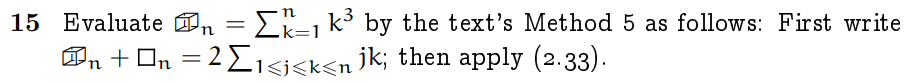
\includegraphics[scale = 1]{Q1.png}
\end{figure}
由2-33,我们令 $a_{k} = k$,于是有:
\begin{align}
    \sum_{k=1}^{n} k^{3} + \sum_{k=1}^{n} k^{2} &= 2(\sum_{1 \le j \le k \le n}jk)\\
    &=(\sum_{k=1}^{n}k)^{2} + \sum_{k=1}^{n}k^2\\
    &=\frac{n^2(n+1)^2}{4} + \sum_{k=1}^{n}k^2
\end{align}
整理等式,两侧消去相同项,得到:
\begin{align}
    \sum_{k=1}^{n}k^3 = \frac{n^2(n+1)^2}{4}
\end{align}

\section*{Basics 16}
\begin{figure}[H]
    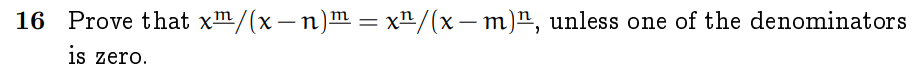
\includegraphics[scale = 1]{Q2.png}
\end{figure}
若两式中有一者分母为零,则显然不成立,下面讨论分母不为零的情况。
\begin{align}
    \frac{x^{\underline{m}}}{(x-n)^{\underline{m}}} &=
    \frac{x(x-1)\cdots(x-m+1)}{(x-n)(x-n-1)\cdots(x-n-m+1)}
\end{align}
若m=n,原式显然成立,不妨令m<n;
\begin{align}
    \frac{x^{\underline{m}}}{(x-n)^{\underline{m}}} &=
    \frac{x(x-1)\cdots(x-m+1)}{(x-n)(x-n-1)\cdots(x-n-m+1)}
    \\
    &=\frac{x(x-1)\cdots(x-m+1)(x-m)\cdots(x-n+1)}{(x-m)(x-m-1)\cdots(x-n+1)(x-n)(x-n-1)\cdots(x-n-m+1)}
    \\
    &=\frac{x^{\underline{n}}}{(x-m)^{\underline{n}}}
\end{align}


\section*{Basics 17}
\begin{figure}[H]
    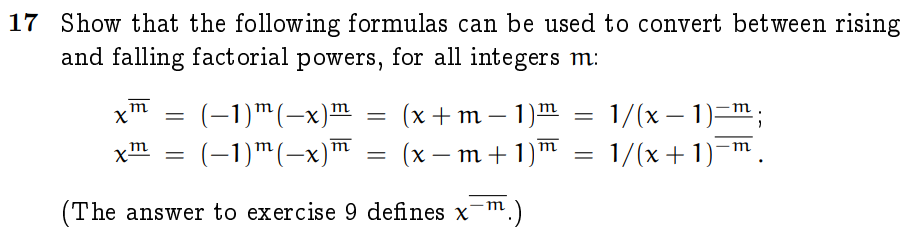
\includegraphics[scale = 1]{Q3.png}
\end{figure}
从左到右进行等价变换,有:
\begin{align}
    x^{\bar{m}} &= x(x+1) \cdots (x+m-1)\\
    % 将每一项都变为相反数,有:\\
    &=(-1)^m(-x)(-x-1) \cdots (-x-m+1)\\
    &=(-x)^{\underline{m}}\\
    &=(x+m-1)(x+m-1-1)\cdots(x+m-1-m+1)\\
    &=(x+m-1)^{\underline{m}}\\
\end{align}
由习题9给出的定义:
\begin{align}
    x^{\bar{m}} &= \frac{1}{(x-1)^{\underline{-m}}}
\end{align}
原式得证。
对于第二个式子,有
\begin{align}
    x^{\underline{m}} &= x(x-1) \cdots (x-m+1)\\
    % 将每一项都变为相反数,有:\\
    &=(-1)^m(-x)(-x+1) \cdots (-x+m-1)\\
    &=(-x)^{\bar{m}}\\
    &=(x-m+1)(x-m+1+1)\cdots(x-m+1=m-1)\\
    &=(x+m-1)^{\bar{m}}\\
\end{align}
由习题9给出的定义:
\begin{align}
    x^{\underline{m}} &= \frac{1}{(x+1)^{\bar{-m}}}
\end{align}
原式得证。


\section*{Basics 18}
\begin{figure}[H]
    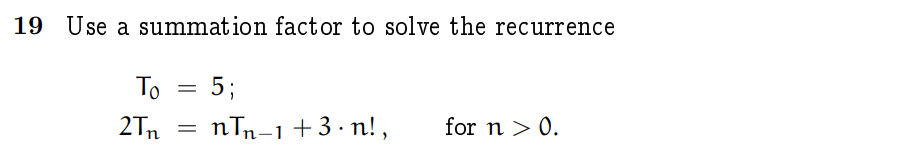
\includegraphics[scale = 1]{Q4.png}
\end{figure}
由求和因子法,不妨令,$a_{n} = 2$,$b_{n} = n$,
我们需要求$s_{n}$,使得:
\begin{equation}
    a_{n-1}s_{n-1} = a_{n}b_{n} 
\end{equation}
得到:
\begin{equation}
    \frac{s_{n}}{s_{n-1}} = \frac{2}{n}
\end{equation}
使用累乘,得到:
\begin{equation}
    s_{n} = \frac{2^{n-1}}{n!}
\end{equation}
故,不妨令$A_{n} = a_{n}s_{n}T_{n}$,
得到:
\begin{equation}
    A_{n} = A_{n-1} + 3\times 2^{n-1}
\end{equation}
累加得到:
\begin{equation}
    A_{n} = 3\times 2^n +5
\end{equation}
最终得到:
\begin{equation}
    T_{n} = 3 \times n! + \frac{n!}{2^{n-1}}
\end{equation}

\end{document}